%!TEX root = ../master.tex
\chapter{Discussion}\label{ch:discussion}
This chapter contains discussion of the entire project.

\section{Sources of error}
Since the final test was conducted on 14 Medialogy students and one Art \& technology student, it is difficult to say whether the product would be just as usable for a regular user. To investigate if the product would be understood amongst users with no knowledge of audio processing, the optimal solution would be testing the product in the proper context. The context in this case could be at an art museum, where the product could be tested on random visitors of all age groups.

From the test facilitators and the secretaries perspective some of the participants answers of whether they were able to hear the difference between the three filters effects were not clear enough. It was indicated that the participants had a doubt if the noise came from the effect applied or the image itself, since the audiolosation of the image could been mistaken for effects. This problem could potentially have been tackled by having an additional test for just the effects by applying them on familiar sounds such as a continuous bell ringing or bird chirping. 

During the testing, when asked if the participants had any further comments to the prototype, a few participants mentioned they could hear the effects better on ‘Trolden og Fuglene’ compared to the ‘Mona Lisa’. This is not to be confused with the results on Tables \ref{tab:comb}, \ref{tab:bandpass}, \ref{tab:highshelf}, whether there is a difference between ‘MAX’ and ‘MIN’ of the three filters on both paintings. It comes down to the whether the image itself and the implementation of the filters has anything to do with how intense the effect itself appears. Since only a few participants had that opinion, there was not enough data to support that claim. It could be useful to actively examine this with interview questions that relate to this.

\section{Wider Context}
During this project, two of the members of the project group spent a day visiting the art museum Kunsten in Aalborg. The goal was to find out how the artefact could be used in context at the museum. With the unfinished prototype in mind, the group members studied the different art exhibitions and tried to imagine the product in context with the art.

During the visit, three exhibitions, as can be seen on Figures \ref{Fig:Kblod}, \ref{Fig:aftryk} and \ref{Fig:chalk}, were considered the main inspiration for the context of use. These images were used to create sketches of the project artefact as a setup in an art museum as seen in Figure \ref{Fig:productsetupsketch}.

\begin{figure}[!h]
\centering
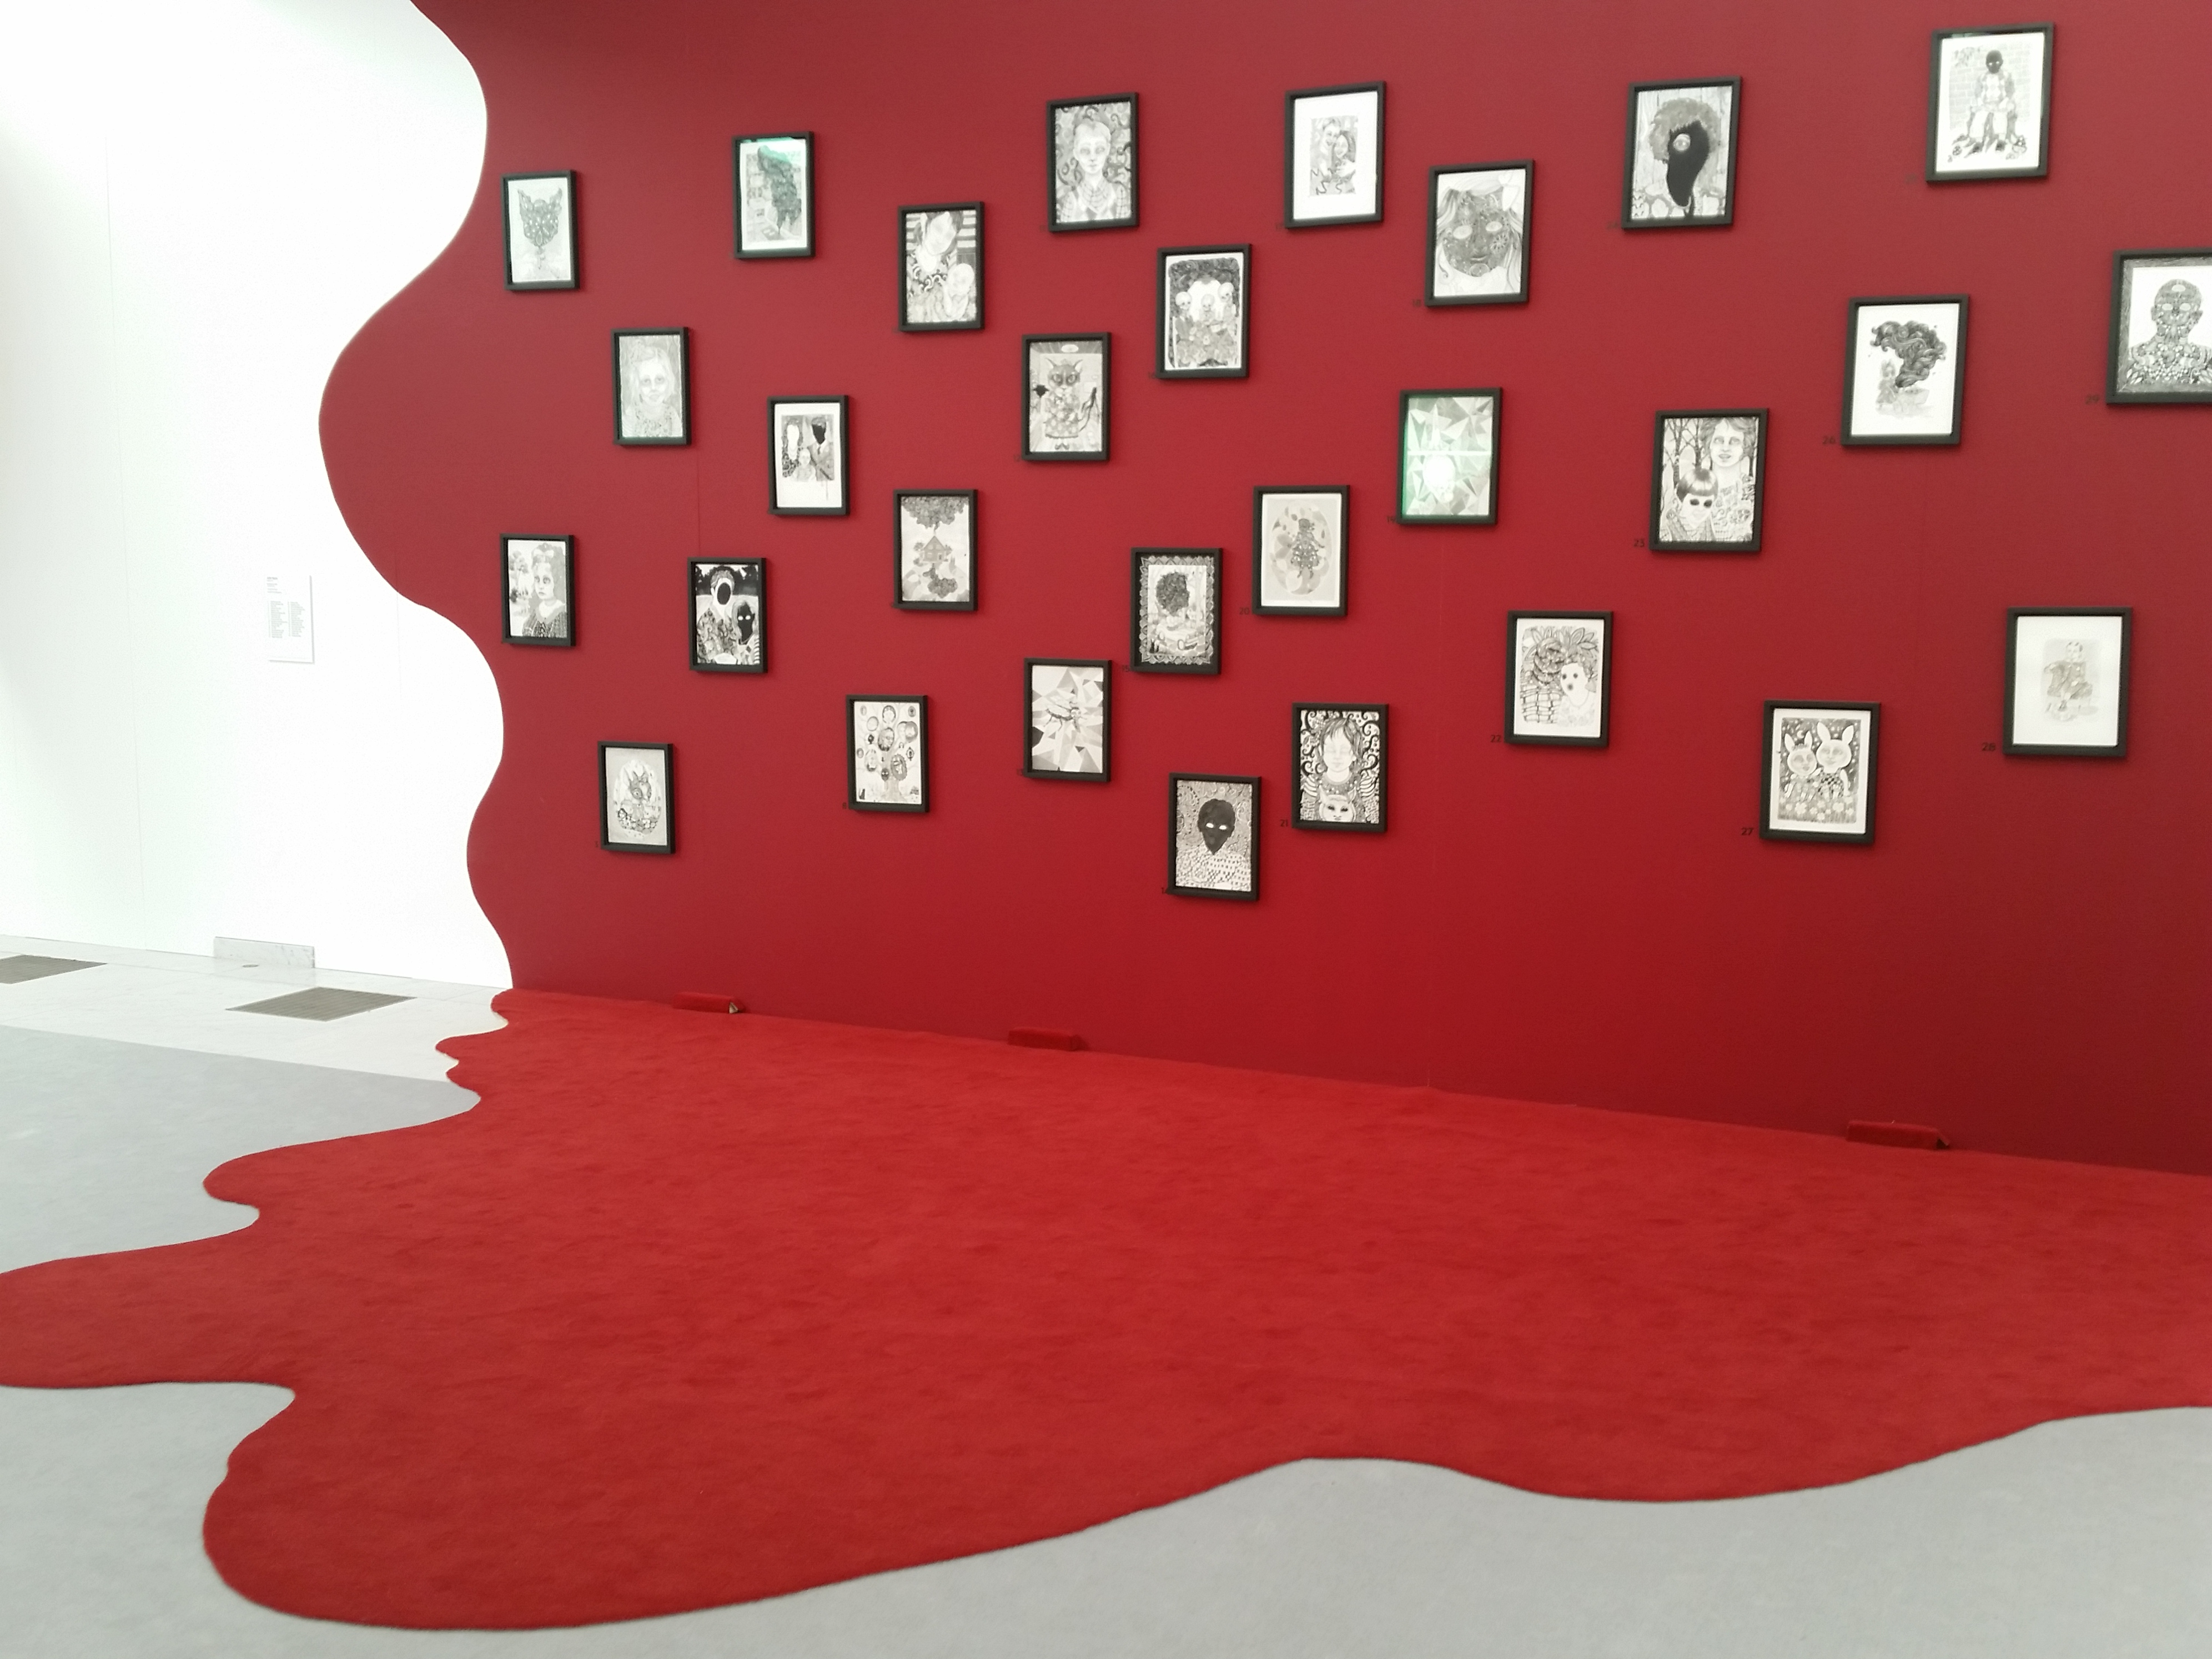
\includegraphics[width=1\textwidth]{Kblod}
\caption{\label{Fig:Kblod} Picture taken from Kunsten.}
\end{figure}
The art piece on Figure \ref{Fig:Kblod} creates a connection between the wall and floor with the red carpet. Inspiration was taken from this piece because the red colour of the floor and wall indicates that the two are connected. The group saw a need to establish an understanding of connectivity between the paint that is being audiolised and the artefact.

\begin{figure}[!h]
\centering
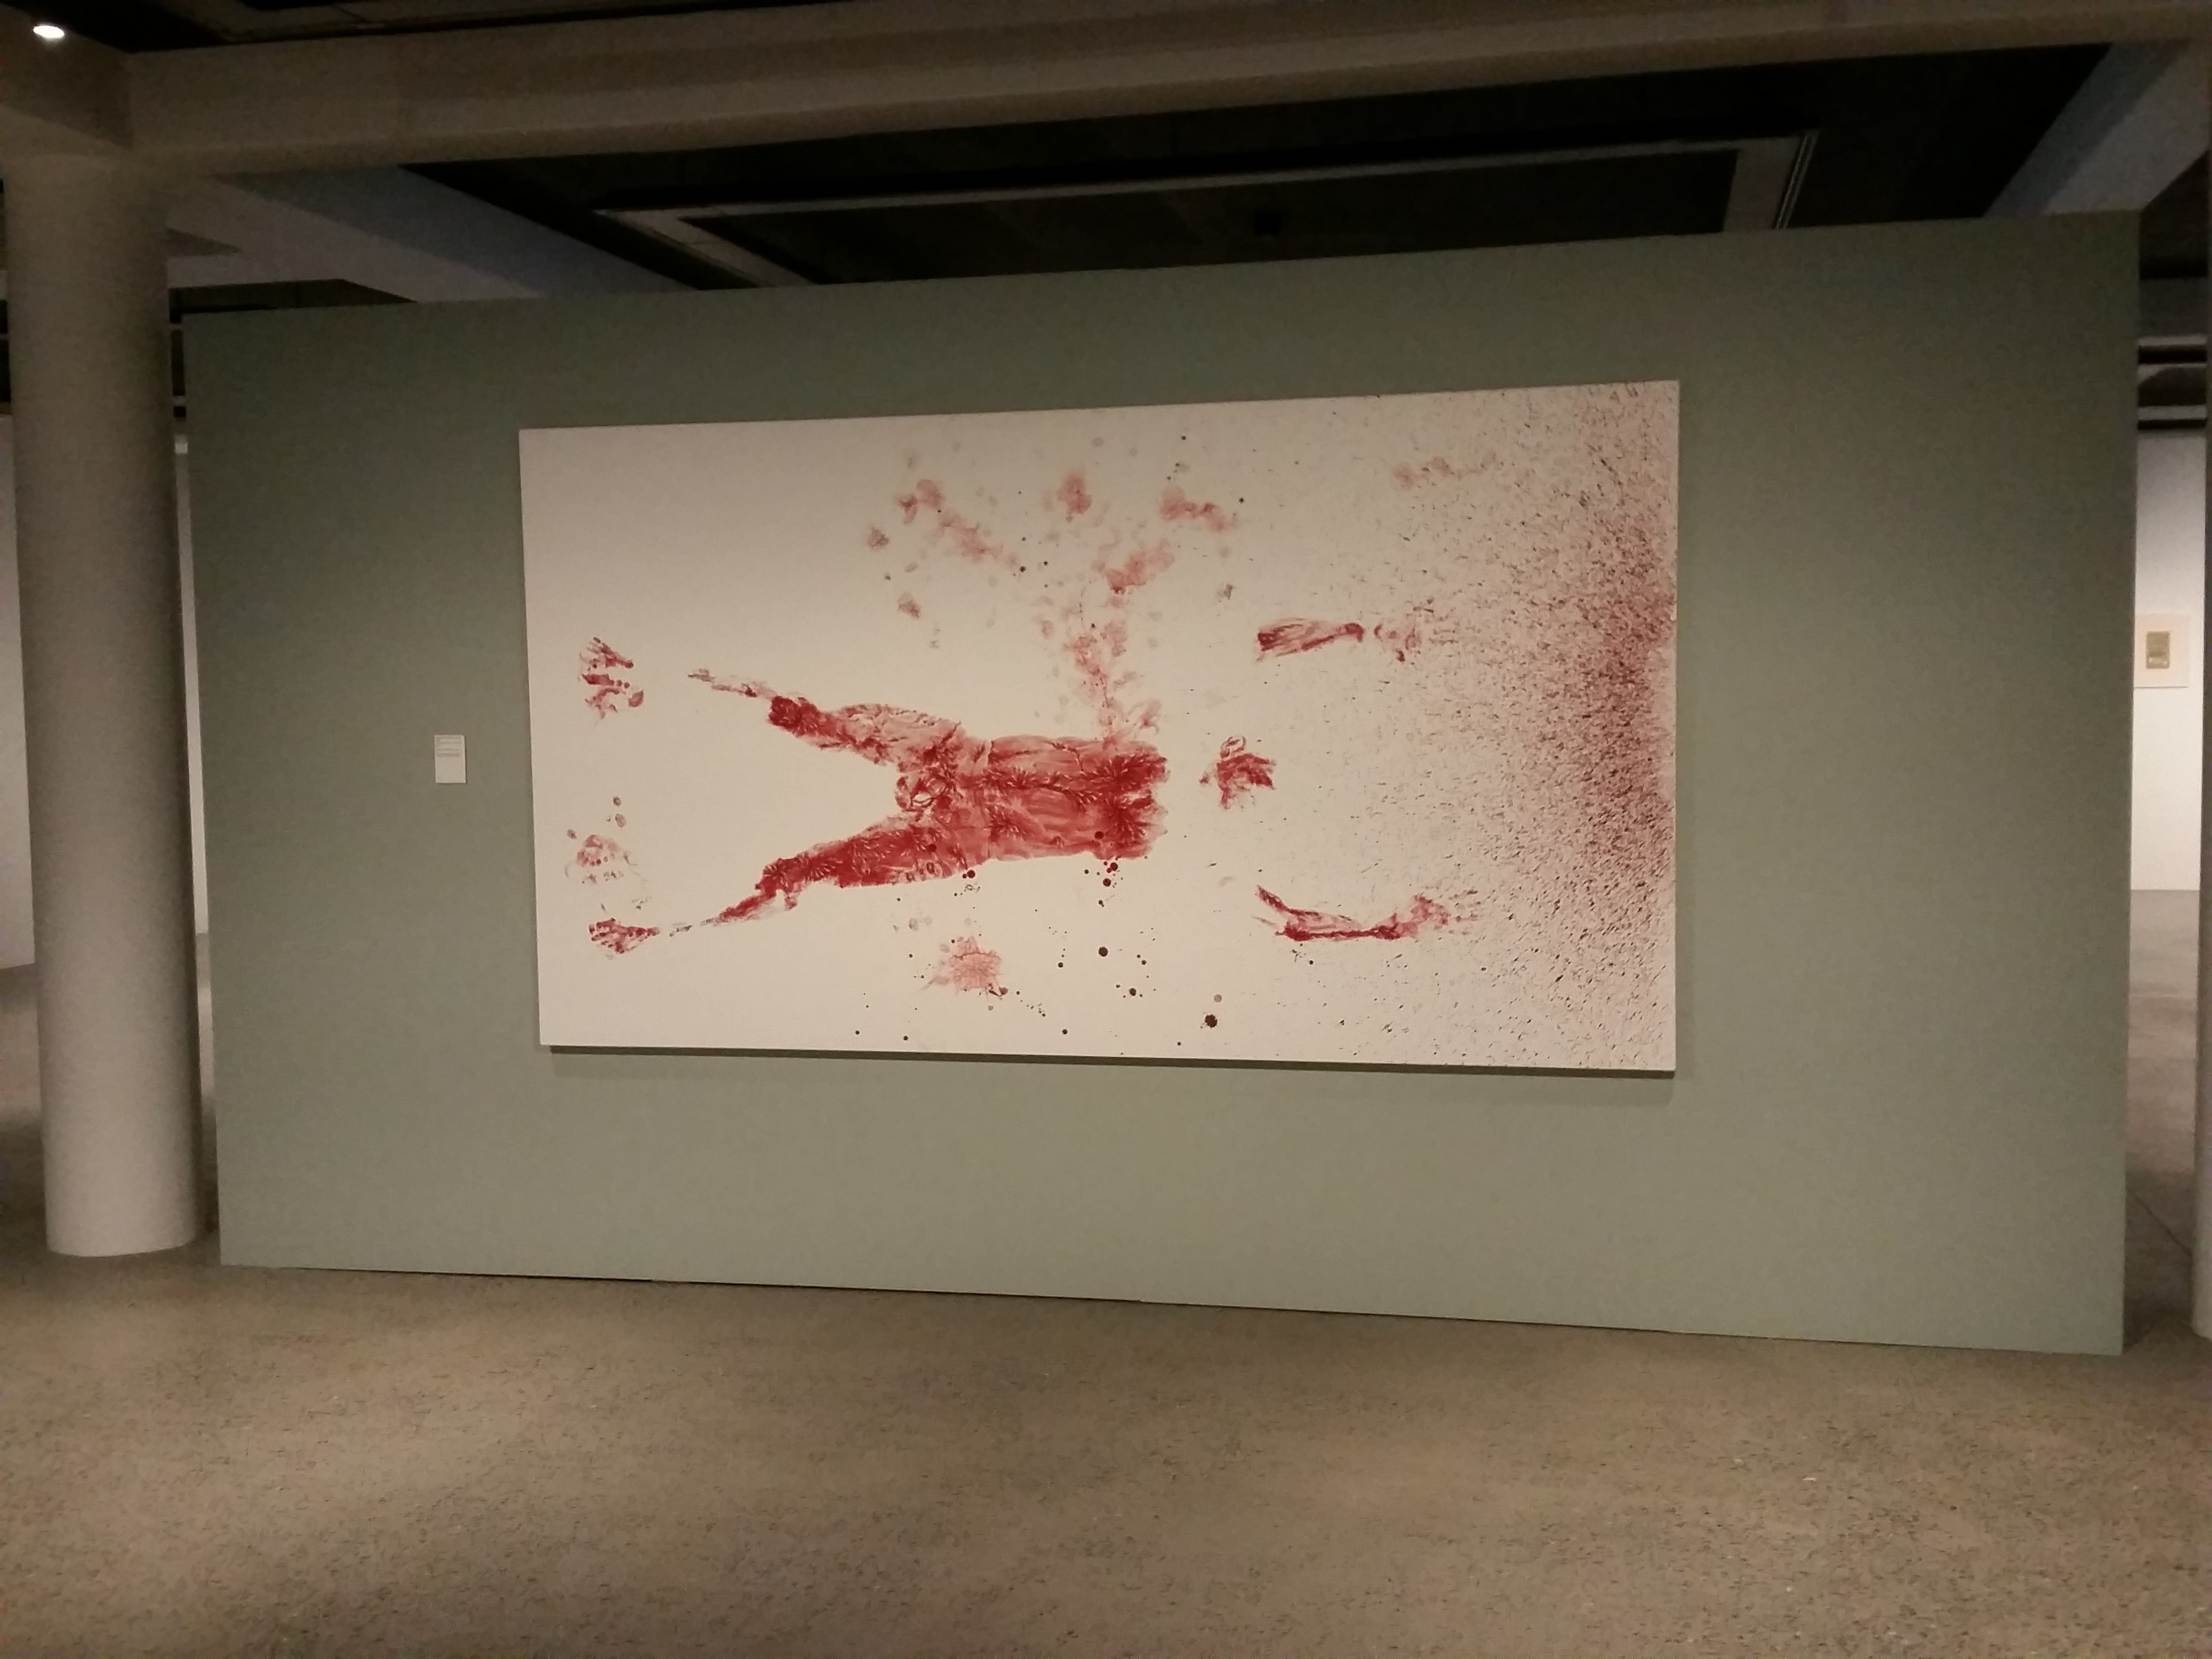
\includegraphics[width=1\textwidth]{aftryk}
\caption{\label{Fig:aftryk} Picture taken from Kunsten.}
\end{figure}

The art piece in Figure \ref{Fig:aftryk} has its own isolated wall with no sharing of space with other art pieces. Since the main project deals with audio, it was decided that it would be optimal for the product to be isolated from other art exhibitions to not disturb the visitors with loud noises.

\begin{figure}[!h]
\centering
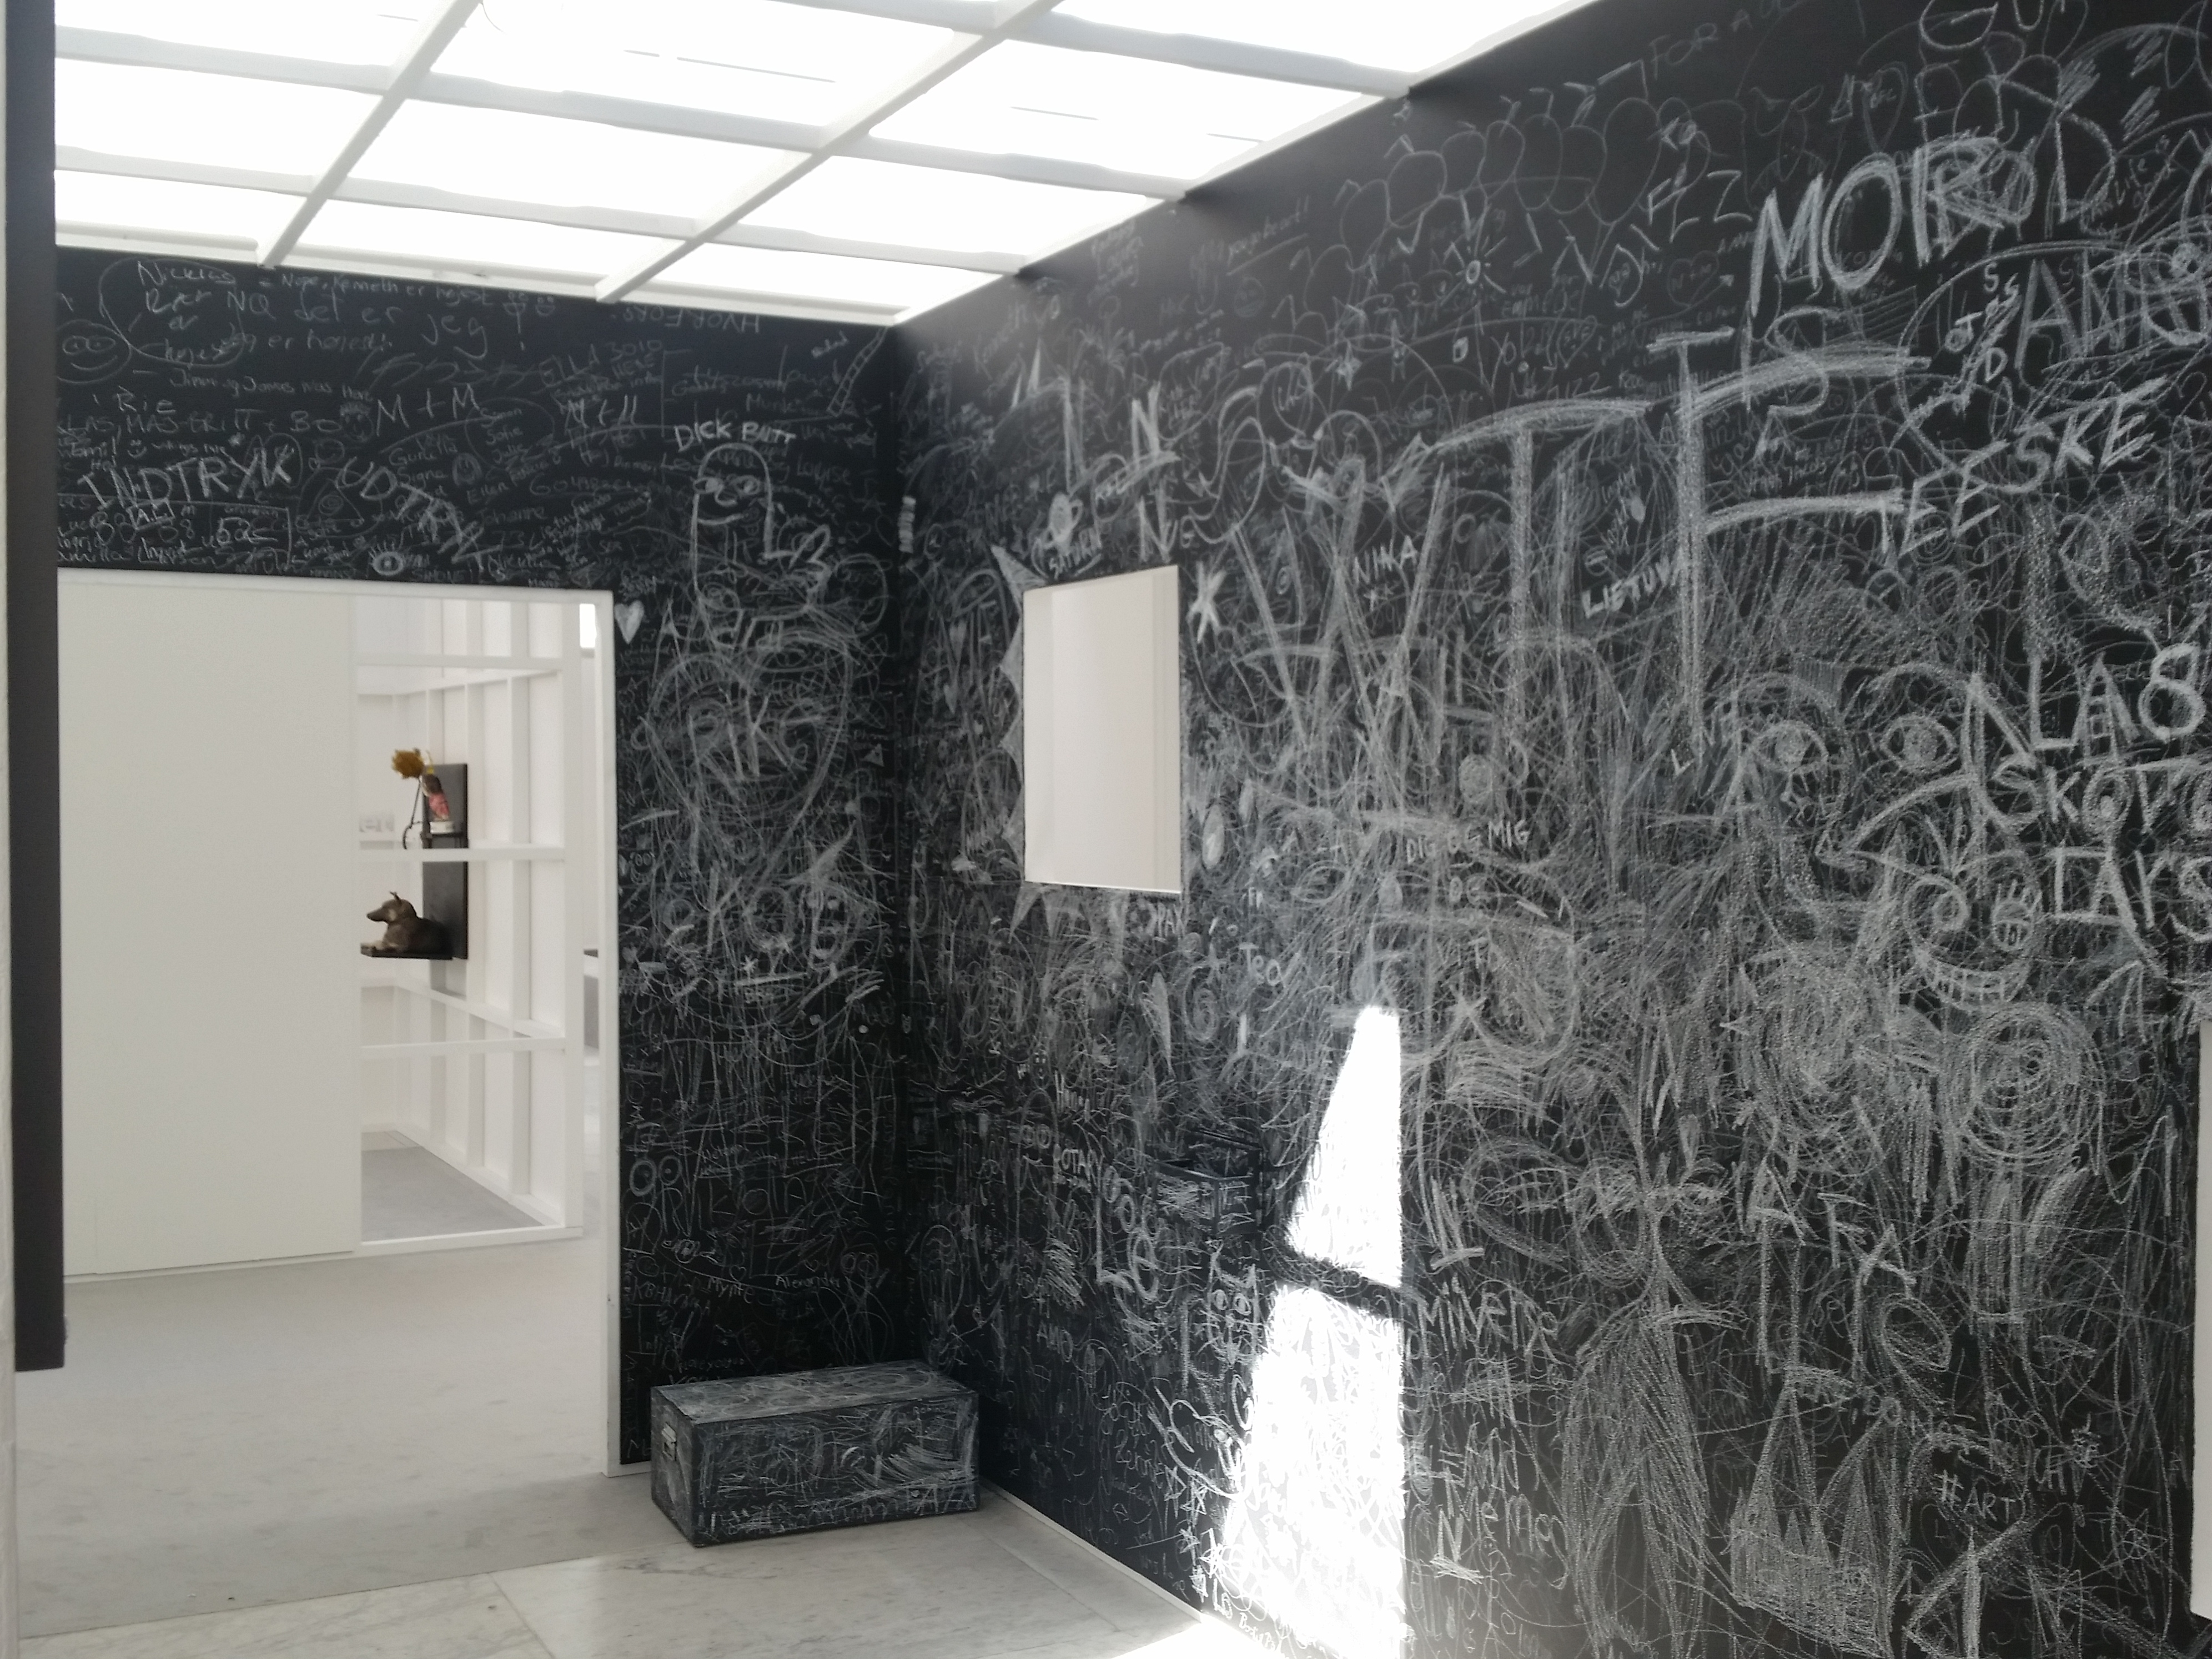
\includegraphics[width=1\textwidth]{chalk}
\caption{\label{Fig:chalk} Picture taken from Kunsten.}
\end{figure}

The interactive art piece seen on Figure \ref{Fig:chalk} is in a closed space and it encourages the visitors to interact with it by drawing on the walls with white chalk. Since the main project is about making the people interact with the product, the group took inspiration from this art piece by looking at its simplistic method of conveying the intended interaction.

The visit at Kunsten resulted in a sketch of how the product could potentially be used in the context of an art museum. The sketch seen on Figure \ref{Fig:productsetupsketch} utilises the colour relationship between the artefact and the painting that is being audiolised as seen in Figure \ref{Fig:Kblod}, the need for isolation from Figure \ref{Fig:aftryk} and lastly a simplistic, interactive design from Figure \ref{Fig:chalk}.

\begin{figure}[!h]
\centering
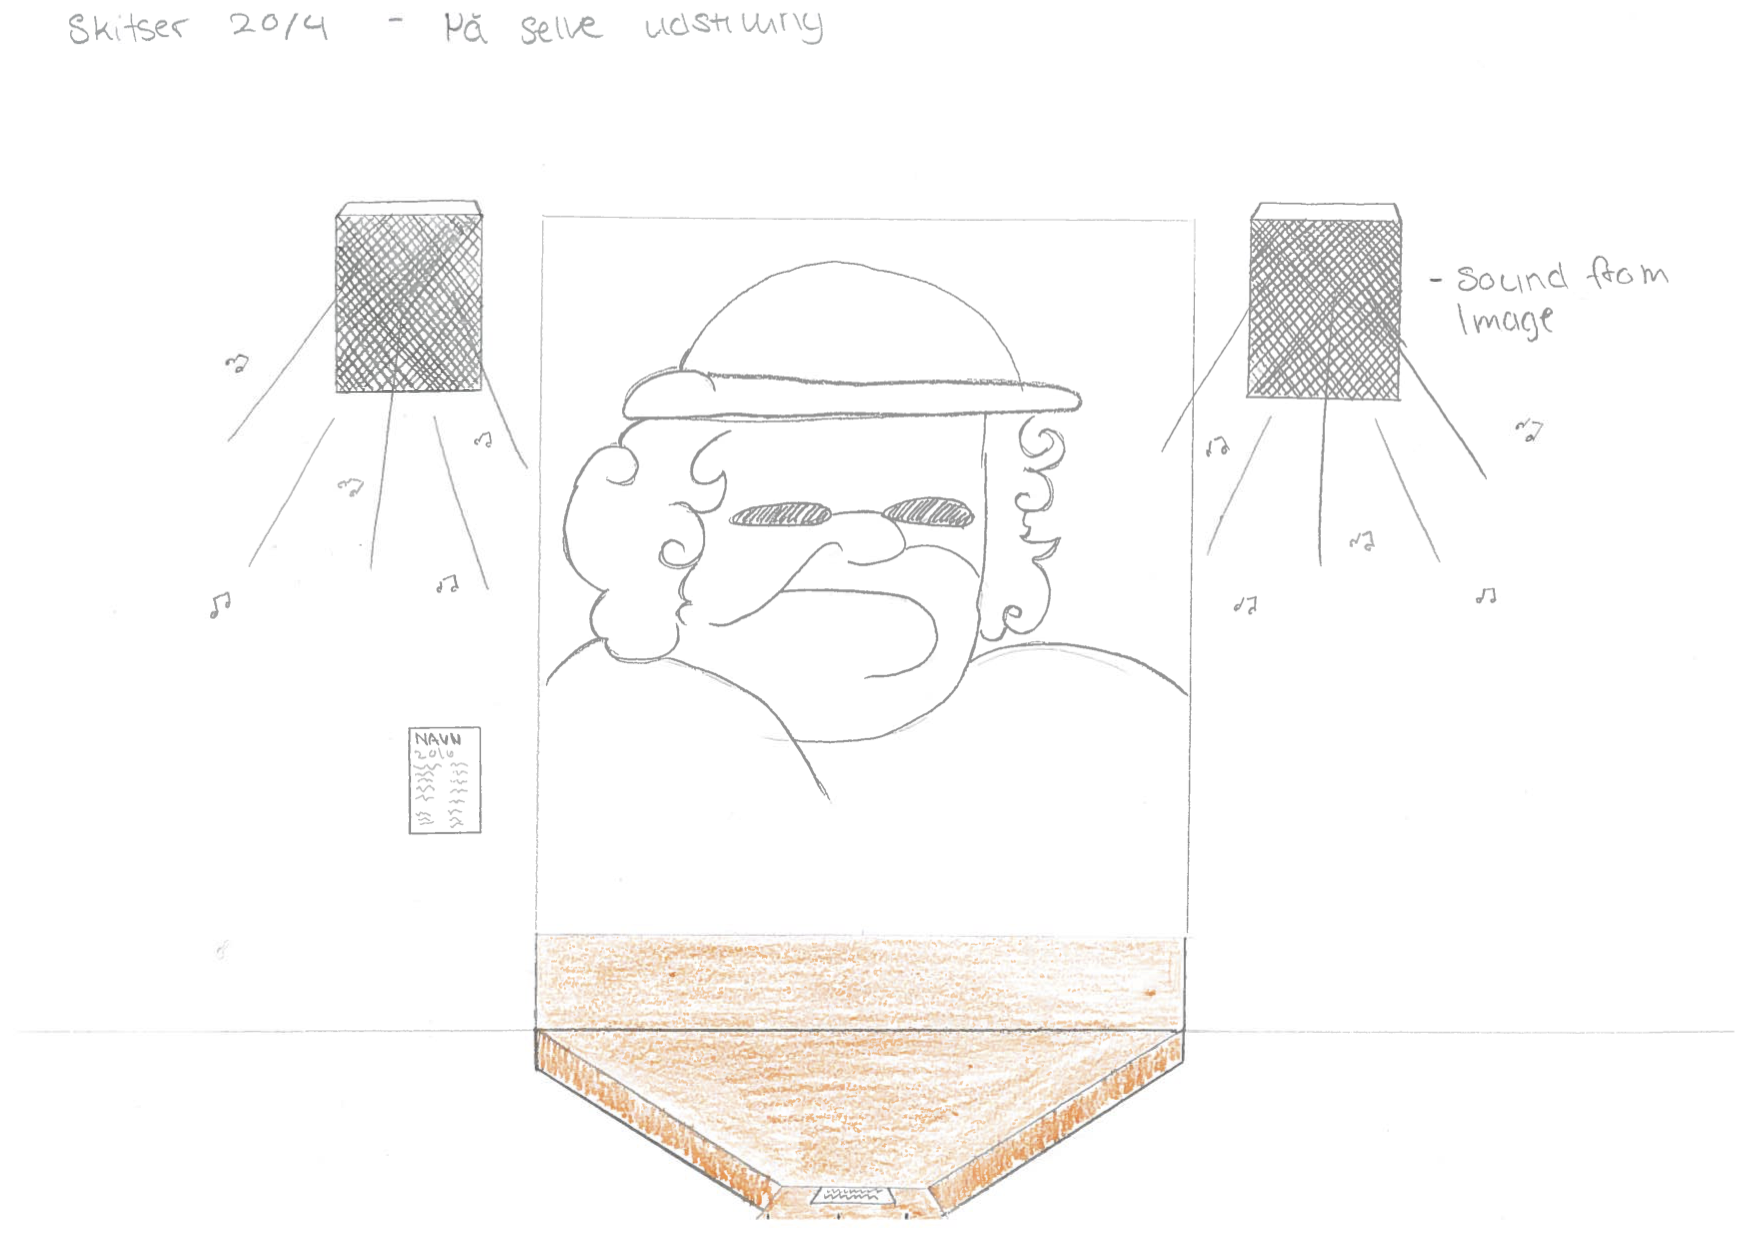
\includegraphics[width=1\textwidth]{productsetupsketch}
\caption{\label{Fig:productsetupsketch} Sketch of an idea, on how to set up the product at an art museum.}
\end{figure}

\section{Further Implementation}
The filters could have been applied differently. Instead of a filter on each colour, the combined signal could have had all filters applied to it in succession. This would produce a more clear effect because each filter would affect the whole signal rather than just part of it. The results might have been different if other filters were used. This could include filters such as reverb, wah-wah, or flanger. These filters could potentially result in an effect that the user could more clearly hear. This also fixes the potential issues that arise if a specific colour channel is not present in an image. If a picture with no green is used, one of the filters is useless, due to it never getting any values. 

Another consideration is the audiolisation. As seen in Chapter~\ref{ch:bgresearch} there are multiple ways of producing sound from an image. The most prevalent of these is using the image as a spectogram where each column or row produces a sample, and each pixel produces an amplitude of a specific frequency in that sample. This could produce a more distinct and interesting sound. 

It is possible to implement the functionality to have the user decide which specific part of the image is currently being audiolised. This would give the user further freedom over the creation of sound, making it more useful as a creative tool. The usability of this needs to be considered, since such an implementation requires more elements in the user interface. This could be achieved using various components such as a joystick, slide potentiometers, or rotary encoders.

Another implementation to consider is allowing for direct manipulation of the audiolised image. This could allow the users to differentiate themselves from each other, and create unique and interesting sounds, increasing its potential as a creative tool for artists as well as non artists. This could also make it an entertaining product to have at festivals, events, or at a museum.

Another alternative version of this product, could be that instead of a picture it worked with a video feed, allowing it to render and manipulate the information given in real-time. This allows the user to translate their surroundings into sounds, giving them a new perspective on the world. If this could be implemented onto a hand-held device, the user would be able to use things such as mobile phones or tablets, which would allow the user to audiolise various areas without the need for large, cumbersome interfaces. The user could also have the possibility to upload their own pictures, videos, or even add their own sounds which are played when audiolising.

The product could be used in other contexts such as at a music- or art festival. If the product should be should be presented at a festival, it would have to be changed to be suitable for the location. This could be achieved by making the product portable by putting it on wheels for easier transportation and by elevating the electronic part of the product to prevent it from taking water and dirt in. This idea is illustrated in Figure \ref{fig:vidreudvikling}.

\begin{figure}[!h]
\centering
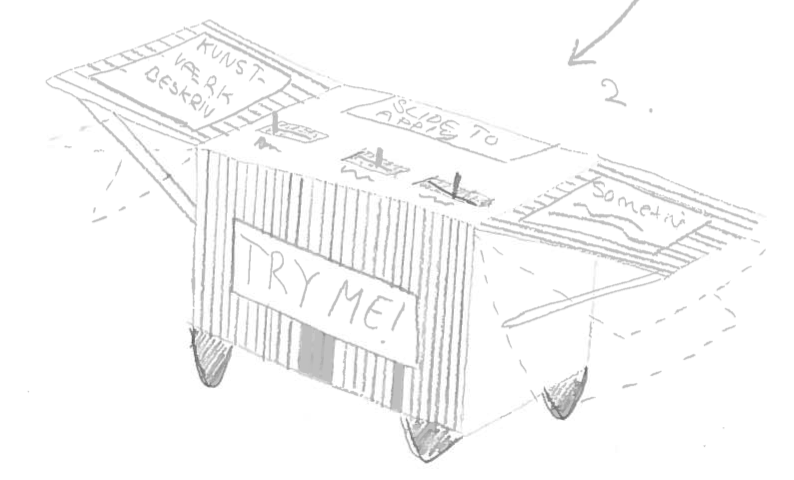
\includegraphics[width=0.5\textwidth]{vidreudvikling}
\caption{\label{fig:vidreudvikling} Sketch of how the portable version could look like.}
\end{figure}

During the final test, one of the test participants was unsure of the connection between the artefact and the paintings shown during the test. He needed clarification of the fact the sound was made by the painting. Ideas were made to visualise the sound on the actual painting like shown in \ref{fig:Visualiseringaflyd}. However, if it is not clear to the user that the image is audiolised, this might just give the impression of an equaliser on top of a picture, confusing the user about what is producing the sound. It is still worth considering, though, that it could make it more clear whether or not an effect is being applied to it. 

\begin{figure}[!h]
\centering
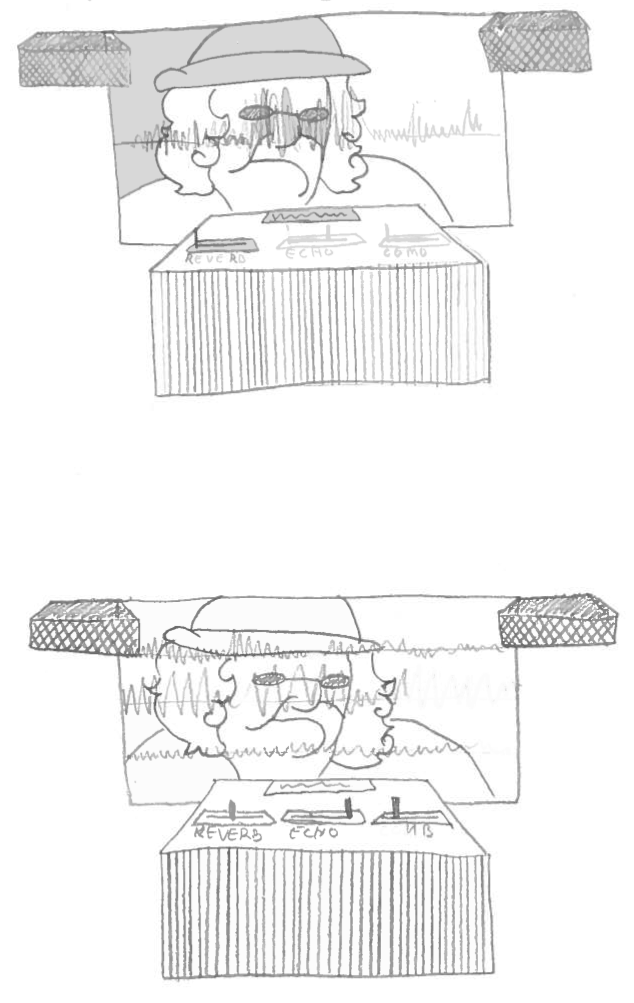
\includegraphics[width=0.5\textwidth]{Visualiseringaflyd}
\caption{\label{fig:Visualiseringaflyd} Sketch on how the sound could be visualised on the image.}
\end{figure}




